\section{Алгоритм быстрого дискретного преобразования для сумм Фурье по ортогональным по Соболеву полиномам, порожденным полиномами Чебышева первого рода}

\subsection{Введение}

В последние десятилетия получила интенсивное развитие теория полиномов, ортогональных относительно скалярного произведения типа Соболева, которые принято называть полиномами, ортогональными  по Соболеву \cite{sms-stn-1-MarcelXu,sms-stn-1-SharIzVuz}. В работе \cite{sms-stn-1-SharIzVuz} были введены и исследованы полиномы $T_{r,k}(x)\,(k=0,1,\ldots)$, ортогональные по Соболеву, порожденные полиномами Чебышева первого рода
%\begin{equation}\label{sms-stn-1-sobcheb1}
$T_0(x)=\frac{1}{\sqrt{2}},\quad T_k(x)=\cos(k\arccos x), \quad k=1,2,\ldots,$
%\end{equation}
посредством следующих равенств
%образующими  ортонормированную  в $L_\mu^2(-1,1)$ с весом  $\mu(x)=\frac2\pi(1-x^2)^{-\frac12}$ систему.

%и выражаются посредством равенств
\begin{equation}\label{sms-stn-1-sobcheb3}
T_{r,k}(x) =\frac{(x+1)^k}{k!}, \quad k=0,1,\ldots, r-1,
\end{equation}
\begin{equation}\label{sms-stn-1-sobcheb4}
T_{r,r}(x) =\frac{(x+1)^r}{\sqrt{2}r!},\quad T_{r,r+n}(x) =\frac{1}{(r-1)!}\int\limits_{-1}^x(x-t)^{r-1}T_{n}(t)dt, \quad n=1,\ldots.
\end{equation}
Эти новые полиномы $T_{r,k}(x)$ ортонормированы \cite{sms-stn-1-SharIzVuz} относительно скалярного произведения
\begin{equation}\label{sms-stn-1-sobcheb2}
\langle f,g\rangle=\sum_{\nu=0}^{r-1}f^{(\nu)}(-1)g^{(\nu)}(-1)+\int_{-1}^{1}f^{(r)}(x)g^{(r)}(x)\mu(x)dx,
\end{equation}
где $\mu(x)=\frac2\pi(1-x^2)^{-\frac12}$.

В \cite{sms-stn-1-SharIzVuz} было показано, что система полиномов $\{T_{r,k}(x)\}_{k=0}^\infty$ образует базис в $W^r_{L^2_\mu(-1,1)}$, кроме того, в \cite{sms-stn-1-SharIzVuz} показано, что ряд Фурье функции $f\in W^r_{L^2_\mu(-1,1)}$ имеет следующий вид
\begin{equation}\label{sms-stn-1-sobcheb7n}
f(x)=\sum_{\nu=0}^{r-1}f^{(\nu)}(-1)\frac{(1+x)^\nu}{\nu!}+ \sum_{k=r}^\infty \hat f_{r,k}T_{r,k}(x),
\end{equation}
где
\begin{equation}\label{sms-stn-1-sobcheb8n}
\hat f_{r,k}=\int_{-1}^1 f^{(r)}(t)T_{k-r}(t)\mu(t)dt,\quad(k\ge r).
\end{equation}
При этом, как показано в \cite{sms-stn-1-SharIzVuz}, ряд Фурье, фигурирующий в правой части равенства \eqref{sms-stn-1-sobcheb7n}, сходится к $f(x)$ равномерно относительно $x\in[-1,1]$.
В частности, при $r=1$ ряд \eqref{sms-stn-1-sobcheb7n} принимает следующий вид:
\begin{equation}\label{sms-stn-1-sobcheb7}
f(x)= f(-1)+ \sum_{k=1}^\infty \hat f_{k}T_{1,k}(x),
\end{equation}
где
\begin{equation}\label{sms-stn-1-sobcheb8}
\hat f_{k}=\int_{-1}^1 f'(t)T_{k-1}(t)\mu(t)dt,\quad(k\ge0).
\end{equation}

Ряды Фурье вида \eqref{sms-stn-1-sobcheb7} встречаются в различных прикладных задачах, в том числе при приближенном решении систем дифференциальных уравнений так называемыми спектральными методами путем применения некоторых итерационных процедур. При этом, в качестве промежуточной возникает необходимость многократного вычисления выражения вида
\begin{equation}\label{sms-stn-1-2.1}
S_N(x) =  S_N(p, x) = \sum\nolimits_{k=0}^{N-1}p_kT_{1,k+1}(x),
\end{equation}
где $p=\{ p_k \}_{k=0}^{N-1}$ -- произвольные действительные числа.

В данном подразделе для решения этой задачи на сетке $x_j=\cos\frac{(2j+1)\pi}{2M}$ $(0\le j\le M-1)$ осуществлен ряд преобразований выражения $S_N(x)$,
которые в итоге позволяют свести рассматриваемую задачу к применению быстрого дискретного преобразования Фурье.
Разработаны соответствующий алгоритм и программа на языке \textbf{C\#}.
С  их помощью проведены численные эксперименты, которые показывают, что алгоритм, основанный на быстром преобразовании
значительно выигрывает в смысле скорости вычислений по сравнению с методом непосредственного вычисления суммы $S_N(x)$ пользуясь явным видом полиномов $T_{1,n}(x)$.

\subsection{Некоторые вспомогательные результаты}

При разработке алгоритма решения этой промежуточной задачи нам понадобятся некоторые преобразования правой части равенства \eqref{sms-stn-1-2.1},
направленные на то, чтобы показать, что при вычислении $S_N(x)$ на сетке %$x_j=\cos\frac{(2j+1)\pi}{2M}$ $(0\le j\le M-1)$
$\{x_j\}_{j=0}^{M-1}$ может быть использовано
быстрое дискретное преобразование Фурье. С этой целью воспользуемся следующими свойствами полиномов $T_{1,k}(x)$, установленными в работе \cite{sms-stn-1-SharIzVuz}:
\begin{equation}\label{sms-stn-1-sobcheb5}
T_{1,0}(x)=1, \quad T_{1,1}(x)=\frac{1+x}{\sqrt{2}}, \quad T_{1,2}(x)=\frac12(x^2-1),
\end{equation}
\begin{equation}\label{sms-stn-1-sobcheb6}
T_{1,k+1}(x)={T_{k+1}(x)\over2(k+1)}- {T_{k-1}(x)\over2(k-1)} -\frac{(-1)^k}{k^2-1},\quad (k\ge 2)
\end{equation}
и запишем  \eqref{sms-stn-1-2.1} в следующем виде
$$
S_N(x)=\frac{p_0}{\sqrt{2}}(1+x)+\frac{p_1}2(x^2-1)+ \sum\nolimits_{k=2}^{N-1}p_k\left[{T_{k+1}(x)\over2(k+1)}- {T_{k-1}(x)\over2(k-1)} -\frac{(-1)^k}{k^2-1}\right]
$$
\begin{multline}\label{sms-stn-1-6.30}
=-\sum\nolimits_{k=2}^{N-1} \frac{(-1)^kp_k}{k^2-1}+\frac{p_0}{\sqrt{2}}(1+x)+\frac{p_1}2(x^2-1)+
\\
\sum\nolimits_{k=2}^{N-1}p_k\left[{T_{k+1}(x)\over2(k+1)}- {T_{k-1}(x)\over2(k-1)}\right].
\end{multline}
Поскольку
$$
\sum\nolimits_{k=2}^{N-1}p_k\left[{T_{k+1}(x)\over2(k+1)}- {T_{k-1}(x)\over2(k-1)} \right]=
\sum\nolimits_{k=2}^{N-1}p_k{T_{k+1}(x)\over2(k+1)}-\sum\nolimits_{k=2}^{N-1}p_k{T_{k-1}(x)\over2(k-1)}=
$$
$$
\sum\nolimits_{k=2}^{N-1}p_k{T_{k+1}(x)\over2(k+1)}-\sum\nolimits_{k=0}^{N-3}p_{k+2}{T_{k+1}(x)\over2(k+1)}=
$$
$$
-{p_{2}\over2}T_{1}(x)-{p_{3}\over4}T_{2}(x)+\sum\nolimits_{k=3}^{N-2}{p_{k-1}-p_{k+1}\over2k}T_k(x)
+{p_{N-2}\over2(N-1)}T_{N-1}(x)+{p_{N-1}\over2N}T_{N}(x),
$$
то   мы можем переписать \eqref{sms-stn-1-6.30} в виде
\begin{multline}\label{sms-stn-1-6.31}
S_N(x)=
\bar p(N)+\frac{p_0}{\sqrt{2}}(1+x)+\frac{p_1}2(x^2-1)-\frac{p_{2}}{2}T_{1}(x)-\frac{p_{3}}{4}T_{2}(x)+
\\
\sum\nolimits_{k=3}^{N-2}\frac{p_{k-1}-p_{k+1}}{2k}T_k(x)
+\frac{p_{N-2}}{2(N-1)}T_{N-1}(x)+\frac{p_{N-1}}{2N}T_{N}(x),
\end{multline}
где
\begin{equation}\label{sms-stn-1-6.32}
\bar p(N)= -\sum\nolimits_{k=2}^{N-1} \frac{(-1)^kp_k}{k^2-1}.
\end{equation}
Далее имеем
$$
\frac{p_0}{\sqrt{2}}(1+x)=p_0T_0+\frac{p_0}{\sqrt{2}}T_1(x), \frac{p_1}2(x^2-1)= \frac{p_1}4T_2(x) -\frac{p_1}{2\sqrt{2}}T_0,
$$
поэтому из \eqref{sms-stn-1-6.31} и  \eqref{sms-stn-1-6.32} окончательно получаем
\begin{multline}\label{sms-stn-1-6.33}
S_N(x)=\bar p(N)+\left(p_0-\frac{p_1}{2\sqrt{2}}\right)T_0+\left(\frac{p_0}{\sqrt{2}}-{p_{2}\over2}\right)T_1(x)+
\\
\sum\nolimits_{k=2}^{N-2}{p_{k-1}-p_{k+1}\over2k}T_k(x)
+{p_{N-2}\over2(N-1)}T_{N-1}(x)+{p_{N-1}\over2N}T_{N}(x).
\end{multline}
Полагая $x=\cos\theta$, это равенство можно переписать
\begin{multline}\label{sms-stn-1-6.34}
Q_N(\theta)=S_N(\cos\theta)=
\bar p(N)+\frac{p_0}{\sqrt{2}}-\frac{p_1}{4}+\left(\frac{p_0}{\sqrt{2}}-{p_{2}\over2}\right)\cos\theta+
\\
\sum\nolimits_{k=2}^{N-2}{p_{k-1}-p_{k+1}\over2k}\cos k\theta
+{p_{N-2}\over2(N-1)}\cos(N-1)\theta+{p_{N-1}\over2N}\cos N\theta.
\end{multline}
Таким образом, вычисление значений алгебраического полинома $S_N(x)$ на сетке $x_j$ $(0\le j\le M-1)$ сводится к вычислению
четного тригонометрического полинома $Q_N(\theta)$ на сетке $\theta_j=\frac{(2j+1)\pi}{2M}$ $(0\le j\le M-1)$, которое можно осуществлять путем быстрого
дискретного косинусного преобразования Фурье. Перейдем к более подробному обсуждению этого вопроса.

\subsection{Описание алгоритма вычисления суммы $S_N(x)$}

В настоящем пункте будет описан алгоритм быстрого дискретного преобразования сумм $S_N(x)$.
Полагая $x=\cos\theta$ и используя \eqref{sms-stn-1-6.34}, мы можем переписать сумму \eqref{sms-stn-1-2.1} в виде следующей суммы по косинусам
\begin{equation}\label{sms-stn-1-sobcheb12}
Q_N(\theta) =
d_{0} + \sum_{k=1}^{N}  d_{k} \cos{k\theta}=S_N(\cos\theta),
\end{equation}
где
\begin{align}
d_{0} =
\bar p(N) + \frac{ p_{0}}{\sqrt{2} }-\frac{ p_{1}}{4},
&\quad
d_{1} =
\frac{ p_{0}}{\sqrt{2}}-\frac{ p_{2}}{2},\label{sms-stn-1-sobcheb13}
\\
d_{k} =
\frac{ p_{k-1}- p_{k+1}}{2k},
&\quad(2 \leq k \leq N-2),\label{sms-stn-1-sobcheb13.1}
\\
d_{N-1} =
\frac{ p_{N-2}}{2(N-1)},
&\quad
d_{N} =
\frac{ p_{N-1}}{2N}.\label{sms-stn-1-sobcheb13.2}
\end{align}

Тогда  значения частичной суммы  \eqref{sms-stn-1-2.1} в узлах $\{x_j = \cos\theta_j\}_{j=0}^{M-1}$ %$(0\le j\le M-1)$
могут быть вычислены с помощью формулы
\begin{equation}\label{sms-stn-1-sobcheb12.a}
Q_N(\theta_j) =
d_{0} + \sum_{k=1}^{N}  d_{k} \cos{k \theta_j}, \quad (0\le j\le M-1).
\end{equation}
Как хорошо известно, эта задача
в случае, когда $M \ge N+1$ и $M=2^{m}$, $m \in \mathbb{N}$,
может быть решена путем применения быстрого косинусного преобразования Фурье, основанного на алгоритме \textit{DCT-II} (см. \cite{sms-stn-1-dctBook}).

Подводя итоги отметим, что алгоритм вычисления суммы $S_N(x)$, определяемой равенством \eqref{sms-stn-1-2.1}, сводится к последовательному осуществлению следующих шагов:

\begin{enumerate}
	\item[1.] \textit{
		На вход алгоритма подаются коэффициенты $p_{k}$;
		%(Например, коэффициенты \eqref{sms-stn-1-sobcheb8} некоторой функции $f(x)$ по системе $T_{1,k}(x)$).
	}
	\item[2.] \textit{
		Отправляясь от коэффициентов $p_{k}$, по формулам \eqref{sms-stn-1-sobcheb13} -- \eqref{sms-stn-1-sobcheb13.2} вычисляются новые коэффициенты $ d_{k}$.
		Тогда исходное выражение \eqref{sms-stn-1-2.1} принимает вид \eqref{sms-stn-1-sobcheb12.a};
	}
	\item[3.] \textit{
		Осуществляется вычисление значений $Q_N(\theta)$ в узлах сетки $\{\theta_j\}_{j=0}^{M-1}$ с помощью быстрого дискретного косинусного преобразования Фурье DCT-II.
	}
\end{enumerate}

\subsection{Численные эксперименты}
Авторами была разработана компьютерная программа, реализующая предложенный алгоритм.

\begin{center}
	\textbf{\textit{Принцип работы с программой}}
\end{center}
\begin{enumerate}
	\item[1.] \textit{
		Пользователь задает количество узлов сетки $N$ и количество $M$ экспериментов, которые он хочет провести.
	}
	\item[2.] \textit{
		Программа генерирует $M$ наборов случайных коэффициентов в задаваемом пользователем диапазоне. Есть возможность отображения сгенерированных коэффициентов.
	}
	\item[3.] \textit{
		Пользователь выбирает --- осуществление обычных либо быстрых преобразований над сгенерированными наборами коэффициентов.
	}
	\item[4.] \textit{
		После осуществления преобразований, программа выводит количество затраченного времени (всего и в среднем на один эксперимент), также средние по всем экспериментам погрешности двух видов --- максмальное отклонение и отклонение в среднем.
		%В качестве проверочных значений используются значения, полученные с помощью длинной арифметики для явных преобразований.
		Имеется возможность отображения подробных сведений об ошибках для каждого эксперимента.
	}
\end{enumerate}

Далее мы приведем несколько скриншотов с пояснениями.

\begin{figure}[H]
	%\centering
	% Requires \usepackage{graphicx}
	\begin{center}
		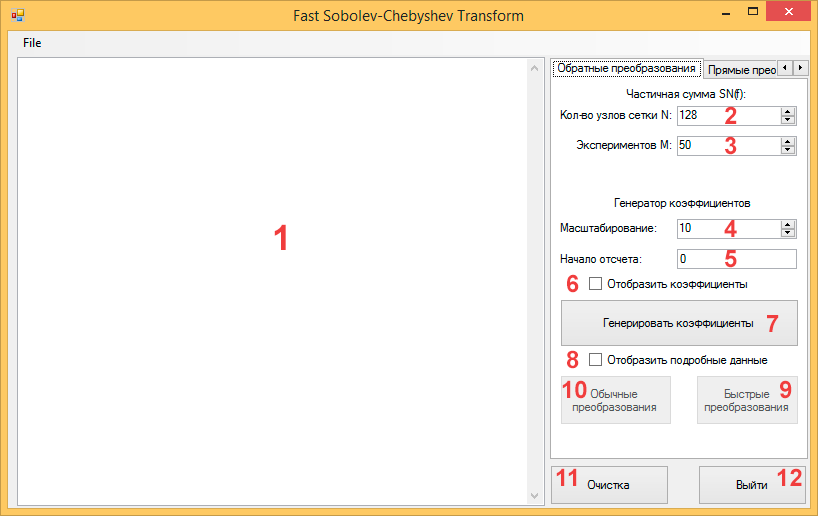
\includegraphics[width=200pt]{pictures/sms-stn-1(1)}\\
		\caption{Главный экран программы}\label{sms-stn-1-img1}
	\end{center}
\end{figure}

Составные части интерфейса (рисунок \ref{sms-stn-1-img1}):

\begin{enumerate}
	\item[1.] Текстовое поле для вывода сообщений программы (<<консоль>>).
	\item[2.] Задание количества узлов сетки $N$. Для осуществления быстрых преобразований требуется чтобы это число было степенью двойки.
	\item[3.] Задание количества экспериментов $M$.
	\item[4.] Задание разброса случайных коэффициентов (дисперсия).
	\item[5.] Задание математического ожидания наборов случайных коэффициентов.
	\item[6.] Служит для выбора -- отображать подробные данные о сгенерированных коэффициентах или нет.
	\item[7.] Генерирование коэффициентов с выбранными параметрами.
	\item[8.] Служит для выбора -- отображать подробные об ошибках в экспериментах или нет.
	\item[9.] Осуществление преобразований по формуле \eqref{sms-stn-1-2.1}.
	\item[10.] Осуществление быстрых преобразований по формуле \eqref{sms-stn-1-sobcheb12.a}.
	\item[11.] Очистка <<консоли>>.
	\item[12.] Выход из программы.
\end{enumerate}

\begin{figure}[H]
	%\centering
	% Requires \usepackage{graphicx}
	\begin{center}
		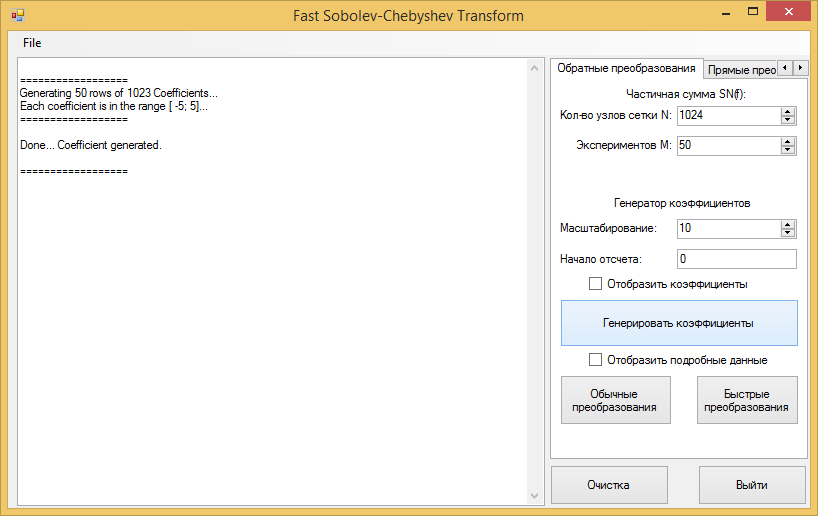
\includegraphics[width=170pt]{pictures/sms-stn-1(2)}
		\quad
		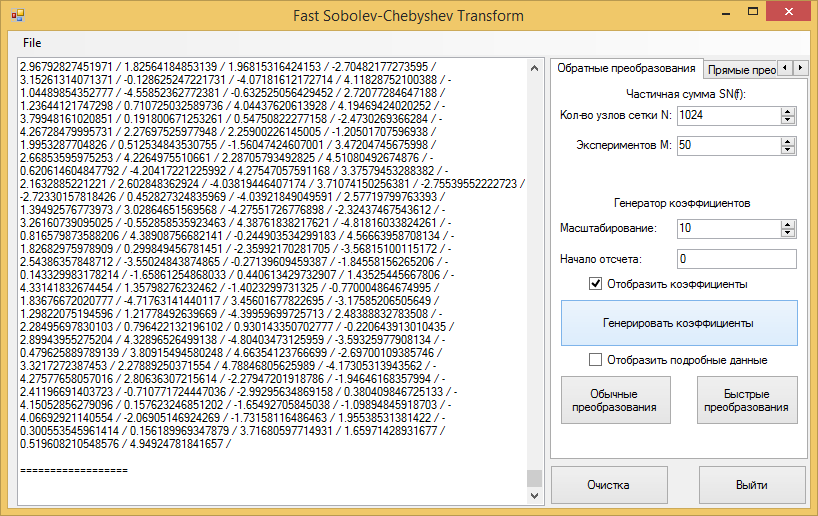
\includegraphics[width=170pt]{pictures/sms-stn-1(3)}
		\caption{
			Сгенерирован набор случайных коэффициентов. Наборов -- 50, количество коэффициентов в каждом -- 1023. Справа --- подробные данные о коэффициентах
		}\label{sms-stn-1-img2}
	\end{center}
\end{figure}

\begin{figure}[H]
	%\centering
	% Requires \usepackage{graphicx}
	\begin{center}
		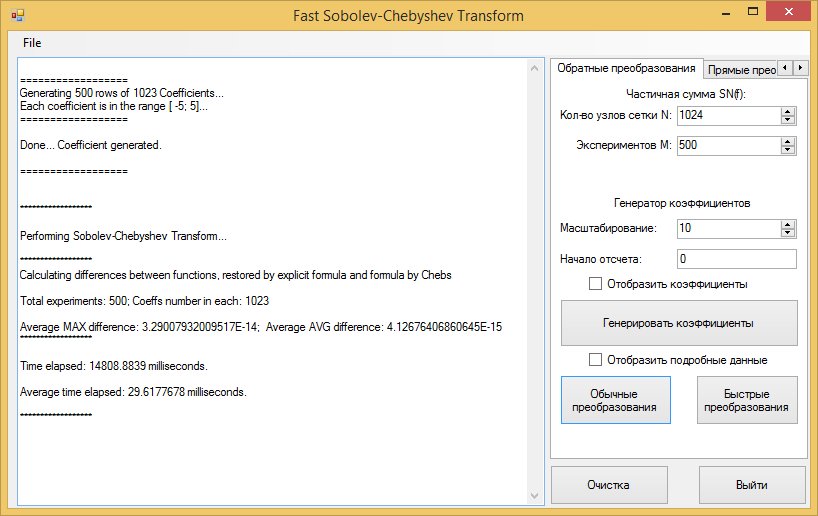
\includegraphics[width=170pt]{pictures/sms-stn-1(4)}
		\quad
		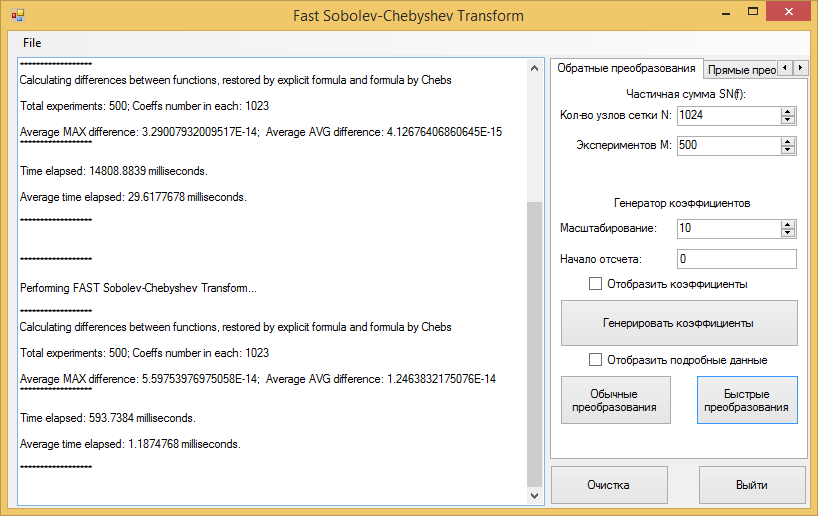
\includegraphics[width=170pt]{pictures/sms-stn-1(5)}
		\caption{
			Осуществлены обычное (слева) и быстрое (справа) преобразования суммы Фурье по системе полиномов $T_{1,k}(x)$
		}\label{sms-stn-1-img3}
	\end{center}
\end{figure}

Проведено 500 экспериментов с 1023 коэффициентами в каждом.
Средняя макси-\linebreak мальная погрешность составила \textit{3.29007932009517E-14}, отклонение в среднем -- \linebreak \textit{4.12676406860645E-15}.
На осуществление всех преобразований затрачено $14808.8839$ миллисекунд (мс), в среднем на эксперимент затрачено $29.6177678$ мс.

Далее, на том же наборе коэффициентов произведены быстрые преобразования.
Средняя максимальная погрешность составила \textit{5.59753976975058E-14}, отклонение в среднем -- \linebreak \textit{1.2463832175076E-14}.
На осуществление всех преобразований затрачено $593.7384$ мс, в среднем на эксперимент затрачено $1.1874768$ мс. Также приведем сравнительную таблицу среднего времени вычисления $S_N(x_j)$ при различных $N$ посредством быстрой и обычной формул в миллисекундах.
%\begin{table}[h!]
%	\centering
%	\begin{tabular}{||c c c ||}
%		\hline
%		\text{Число узлов} & \text{Обычная формула} & \text{С использованием БПФ} \\ [0.5ex]
%		\hline\hline
%		8 		& 0.00225264	& 0.00704127  \\
%		16 		& 0.00647647	& 0.01316473  \\
%		32 		& 0.02033089	& 0.02625329  \\
%		64 		& 0.06989277	& 0.0542377   \\
%		128 	& 0.28020358	& 0.12493092   \\
%		256 	& 1.15891625	& 0.27047539   \\
%		512 	& 6.80259062	& 0.61383475   \\
%		1024 	& 37.28032723	& 1.0818284   \\
%		2048 	& 147.88811337	& 2.42418507   \\
%		4096 	& 714.4442895	& 4.8854531   \\
%		\hline
%	\end{tabular}
%\end{table}

%\subsection{Листинг программы}
%
%В этом разделе мы приводим листинг основных функциональных частей разработанной программы.
%
%\vskip0.5cm
%
%\noindent\textit{
%	Основные функции \textbf{SobCheb1Benchmark} и \textbf{SobCheb1Benchmark\_Fast},  осуществляющие обычное
%	и быстрое преобразования соответственно и вычисляющие погрешности и затраченное время
%}
%%{\scriptsize
%%	\begin{lstlisting}
%%	public static bool SobCheb1Benchmark(double[] F, out double avg,
%%	out double max, out TimeSpan time)
%%	{
%%	//Вычисление преобразования по явным формулам
%%	//Используется для сравнения и нахождения ошибок
%%	double[] f_expl = SobCheb1RestoreExplicit(F);
%%	
%%	//Вычисление по формуле (2.6), без быстрых преобразований
%%	Stopwatch sw = new Stopwatch();
%%	sw.Start();
%%	double[] f_cheb = SobCheb1Restore(F);
%%	sw.Stop();
%%	time = sw.Elapsed;
%%	
%%	//Вычисляем погрешности
%%	return
%%	MathTools.ArrayDifference(f_expl, f_cheb, out avg, out max);
%%	}
%%	
%%	public static bool SobCheb1Benchmark_Fast(double[] F, out double avg,
%%	out double max, out TimeSpan time)
%%	{
%%	//Вычисление преобразования по явным формулам
%%	//Используется для сравнения и нахождения ошибок
%%	double[] f_expl = SobCheb1RestoreExplicit(F);
%%	
%%	//Быстрое преобразование
%%	Stopwatch sw = new Stopwatch();
%%	sw.Start();
%%	double[] f_cheb = SobCheb1Restore_Fast(F);
%%	sw.Stop();
%%	time = sw.Elapsed;
%%	
%%	//Вычисляем погрешности
%%	return
%%	MathTools.ArrayDifference(f_expl, f_cheb, out avg, out max);
%%	}
%%	
%%	
%%	\end{lstlisting}
%%}
%
%
%\noindent\textit{Для перехода к новым коэффициентам используется функция}
%
%%{\scriptsize
%%	\begin{lstlisting}
%%	static double[] prepareChebCoeffs(double[] F)
%%	{
%%	int N = F.GetLength(0)+1;
%%	int n = N - 1;
%%	double pN = 0.0;
%%	for (int k = 2; k < n; k++) {
%%	pN += MathTools.MinusOne(k) * F[k] / (k * k - 1.0);
%%	}
%%	pN = -pN;
%%	
%%	double[] D = new double[N];
%%	double Sqrt2 = Math.Sqrt(2);
%%	D[0] = F[0] / Sqrt2 - F[1] * 0.25 + pN;
%%	
%%	if (n < 3) {
%%	D[1] = F[0] / Sqrt2;
%%	} else {
%%	D[1] = F[0] / Sqrt2 - 0.5 * F[2];
%%	}
%%	if (n > 1) {
%%	for (int k = 2; k < n - 1; k++)
%%	D[k] = (F[k-1] - F[k + 1]) / (2.0 * k);
%%	}
%%	if (n > 2) {
%%	D[n - 1] = F[n - 2] / (2.0 * n - 2.0);
%%	}
%%	D[n] = F[n-1] / (2.0 * n);
%%	
%%	return D;
%%	}
%%	
%%	\end{lstlisting}
%%}
%
%\noindent\textit{Для вычисления полиномов, ортогональных в смысле Соболева, применяется функция}
%
%%{\scriptsize
%%	\begin{lstlisting}
%%	public static double[][] SobCheb1Normed(double[] t, int m = -1)
%%	{
%%	int N = t.Length;
%%	if (m < 2) { m = N; }
%%	
%%	double tmp = 1.0 / Math.Sqrt(2);
%%	double[][] T1r = new double[m + 1][];
%%	T1r[0] = new double[N];
%%	T1r[1] = new double[N];
%%	T1r[2] = new double[N];
%%	
%%	//Вычисляем T10, T11 and T12
%%	for (int j = 0; j < N; j++) {
%%	T1r[0][j] = 1.0;
%%	T1r[1][j] = tmp * (1.0 + t[j]);
%%	T1r[2][j] = 0.5 * (t[j] * t[j] - 1.0);
%%	}
%%	
%%	//Вычисляем T1k, k >= 3
%%	double[][] T = Cheb1Normed(t, m); //полиномы Чебышева Tn
%%	double c1, c2, c3;
%%	
%%	for (int k = 3; k <= m; k++) {
%%	T1r[k] = new double[N];
%%	//расчет коэффициентов
%%	c1 = 0.5 / (double)k; c2 = 0.5 / (k - 2.0);
%%	if (k % 2 == 0) {
%%	c3 = 1.0 / (double)k / (k - 2.0);
%%	} else {
%%	c3 = -1.0 / (double)k / (k - 2.0);
%%	}
%%	
%%	//основной цикл вычислений
%%	for (int j = 0; j < N; j++) {
%%	T1r[k][j] = c1 * T[k][j] - c2 * T[k - 2][j] + c3;
%%	}
%%	}
%%	
%%	return T1r;
%%	}
%%	\end{lstlisting}
%%}
%
%\noindent\textit{Для вычисления значений частичной суммы $S_N(f,x)$ быстрым и обычным способом служат функции:}
%
%%{\scriptsize
%%	\begin{lstlisting}
%%	public static double[] SobCheb1Restore(double[] F, double[] t = null)
%%	{
%%	int N = F.GetLength(0)+1;
%%	int n = N - 1;
%%	
%%	//Генерирование сетки
%%	if (t == null) {
%%	t = GridGenerator.GetChebZeroes(N);
%%	} else {
%%	N = t.Length;
%%	}
%%	
%%	//Подготовка коэффициентов
%%	double[] D = prepareChebCoeffs(F);
%%	D[0] *= Math.Sqrt(2);
%%	
%%	//Восстановление
%%	double[] Result = Cheb.RestoreCheb1NormedSum(D, t);
%%	
%%	return Result;
%%	}
%%	
%%	
%%	public static double[] SobCheb1Restore_Fast(double[] F)
%%	{
%%	//Подготовка коэффициентов
%%	double[] D = SobCheb.prepareChebCoeffs(F);
%%	
%%	//Восстановление
%%	double[] Result = Cheb.RestoreCheb1NormedSum_Fast(D);
%%	
%%	return Result;
%%	}
%%	\end{lstlisting}
%%}
%
%Кроме того, программа включает классы \textit{\textbf{Cheb}}, \textit{\textbf{FFT}}, \textit{\textbf{DCT}}, \textit{\textbf{IDCT}} и ряд других, используемые внутри указанных функций в качестве служебных,
%а также класс \textit{\textbf{GridGenerator}} для генерации случайных коэффициентов и различных сеток (нулей многочлена Чебышева и его производных и др.).


% TODO Написать заключение